\documentclass[13.5pt,aspecratio=169]{beamer}
\usepackage{graphicx} % Required for inserting images
\usepackage{amsfonts}
\usepackage{amsmath}
\usepackage{amssymb}
\usepackage{physics}
\usepackage{bm}
\usepackage{physics}
\usepackage{booktabs}
\usetheme{Madrid}

\DeclareMathOperator*{\argmax}{arg\,max}
\DeclareMathOperator*{\argmin}{arg\,min}
\graphicspath{{Images/}{./}} 
\usetheme{Copenhagen}
%\usecolortheme{beaver}
\title{CHAPTER 3: N-gram Language Models}
\author[Group 5]{\textit{Instructor: PhD. Nguyen Thi Quy}\\ \bigskip \textbf{Group 5: 3.4 - 3.5}}
\date{\today}
\setbeamertemplate{navigation symbols}{}
\setbeamertemplate{headline}{}
\setbeamercolor{huge text}{fg=white}
%\setbeamercovered{transparent}
\setbeamertemplate{footline}{
    \leavevmode%
    \hbox{%
        \begin{beamercolorbox}[wd=.333333\paperwidth,ht=2.25ex,dp=1ex,center]{author in head/foot}%
            \usebeamerfont{author in head/foot}\insertshortauthor
        \end{beamercolorbox}%
        \begin{beamercolorbox}[wd=.333333\paperwidth,ht=2.25ex,dp=1ex,center]{title in head/foot}%
            \usebeamerfont{title in head/foot}\insertshorttitle
        \end{beamercolorbox}%
        \begin{beamercolorbox}[wd=.333333\paperwidth,ht=2.25ex,dp=1ex,right]{date in head/foot}%
            \usebeamerfont{date in head/foot}\insertshortdate{}\hspace*{2em}
            \insertframenumber{} / \inserttotalframenumber\hspace*{2ex} 
        \end{beamercolorbox}%
    }%
    \vskip0pt%
}

\begin{document}
\maketitle

% \begin{frame}
% 	\frametitle{Table of Contents} % Slide title, remove this command for no title
% 	\tableofcontents[subsectionstyle=hide]
% \end{frame}
%-------------------------------------------------------------------%

\section{3.4: Generalization and Zeros}
% \begin{frame}
% 	\frametitle{Table of Contents} % Slide title, remove this command for no title
% 	\tableofcontents[currentsection, subsectionstyle=hide]
% \end{frame}

\begin{frame}
    \bigskip
    \color{blue} \Huge \textbf{5.4 Generalization and Zeros} 
\end{frame}

%-------------------------------------------------------------------%

\section{3.5: Smoothing} % Sections are added in order to organize your presentation into discrete blocks, all sections and subsections are automatically output to the table of contents as an overview of the talk but NOT output in the presentation as separate slides
% \begin{frame}
% 	\frametitle{Presentation Overview} % Slide title, remove this command for no title
% 	\tableofcontents[currentsection, subsectionstyle=hide]
% \end{frame}
\subsection{Laplace Smoothing}
\begin{frame}
    \bigskip
    \color{blue} \Huge \textbf{3.5 Smoothing} 
\end{frame}

%------------------------------------------------

\begin{frame}
	\frametitle{The intuition of smoothing}
    \begin{minipage}{0.45\textwidth}  % Adjust the width as needed
        \begin{block}{When we have sparse statistics:} % Block without title
            \hspace{30} $P(w \hspace{2} | \hspace{2} \text{denied the})$ \\
            \hspace{35} 3 allegations \\
            \hspace{35} 2 reports \\
            \hspace{35} 1 claims \\
            \hspace{35} 1 request \\
            \hspace{35} 7 total
        \end{block}
    \end{minipage}\hspace{10}
    \begin{minipage}{0.45\textwidth}  % Adjust the width as needed
            \centering
            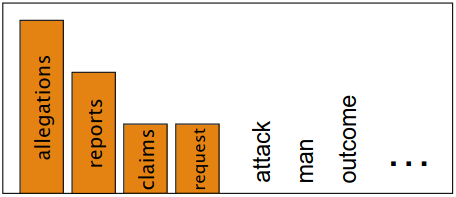
\includegraphics[scale=0.5]{sparse_statistics.png}
    \end{minipage}

    \begin{minipage}{0.45\textwidth}  % Adjust the width as needed
        \begin{block}{Steal probability mass} % Block without title
            \hspace{30} $P(w \hspace{2} | \hspace{2} \text{denied the})$ \\
            \hspace{35} 2.5 allegations \\
            \hspace{35} 1.5 reports \\
            \hspace{35} 0.5 claims \\
            \hspace{35} 0.5 request \\
            \hspace{35} 2 request \\
            \hspace{35} 7 total
        \end{block}
    \end{minipage}\hspace{10}
    \begin{minipage}{0.45\textwidth}  % Adjust the width as needed
            \centering
            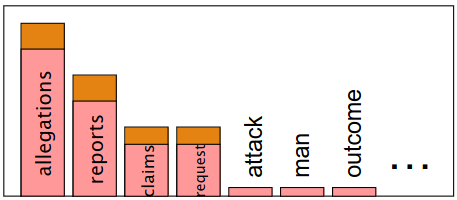
\includegraphics[scale=0.5]{steal_probability_mass.png}
    \end{minipage}
	

\end{frame}


%------------------------------------------------



\begin{frame}
    \onehalfspacing
        \frametitle{Add-one estimation}
        
        {\Large Unsmoothed maximum likelihood estimate} \vspace{-2em}
        {\Large
        \begin{center} 
            \[ P(w_i) = \frac{c_i}{N} \]
        \end{center}
        }
        {\Large Laplace smoothing merely adds one to each count:} \vspace{-2em}
        {\Large
        \begin{center} 
            \[ P_{Laplace} (w_i) = \frac{c_i + 1}{N + V} \]
        \end{center}
        }
\end{frame}
    
%------------------------------------------------

\begin{frame}
    \onehalfspacing
        \frametitle{Add-one estimation}
        
        {\Large It is convenient to describe how a smoothing algorithm affects the numerator, by defining an adjusted count $c^*$: 
        } \vspace{-2em}
        {\Large
        \begin{center} 
            \[ c^*_i = (c_i + 1) \frac{N}{N + V} \]
        \end{center}
        }

        \begin{block}{}
            A related way to view smoothing is as discounting (lowering) some non-zero counts in order to get the probability mass that will be assigned to the zero counts: 
        \end{block} \vspace{-2em}
        {\Large
        \begin{center} 
            \[ d_c = \frac{c^*}{c} \]
        \end{center}
        }
\end{frame}

%------------------------------------------------


\begin{frame}
\onehalfspacing
	\frametitle{Add-one estimation}
	
    {\Large Also called Laplace smoothing}
    \begin{block}{}
        Pretend we saw each word one more time than we did
Just add one to all the counts!
    \end{block}
    \begin{itemize}
        \item MLE estimate:  
        \vspace{-2em}
        \begin{center} 
            \[ P_{MLE}(w_i | w_{i-1}) = \frac{c(w_{i-1}, w_i)}{c(w_{i-1})} \]
          \end{center}
        \item Add-1 estimate:
        \vspace{-2em}
        \begin{center} 
            \[ P_{Add-1}(w_i | w_{i-1}) = \frac{c(w_{i-1}, w_i) + 1}{c(w_{i-1}) + V} \]
          \end{center}
    \end{itemize}
\end{frame}

%------------------------------------------------
\begin{frame}
    \onehalfspacing
        \frametitle{Berkeley Restaurant Corpus}
        \begin{minipage}{0.3\textwidth}
            \begin{block}{}
                \item Raw bigram counts
            \end{block}
        \end{minipage}
        
        \bigskip
            \begin{figure}
                \centering
                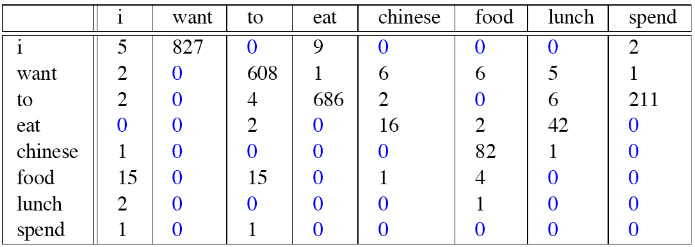
\includegraphics [scale=0.6] {raw_bigram_counts.png}
                \caption{Bigram counts for eight of the words (out of V = 1446) in the Berkeley Restau-
                rant Project corpus of 9332 sentences. Zero counts are in gray.}
            \end{figure}
        
\end{frame}
%------------------------------------------------



%------------------------------------------------
% \begin{frame}
% \onehalfspacing
% 	\frametitle{Maximum Likelihood Estimates}
%     \begin{block}{The maximum likelihood estimate} % Block without title
% 		\begin{itemize}
%             \item of some parameter of a model M from a training set T
%             \item maximizes the likelihood of the training set T given the model M
%         \end{itemize}
% 	\end{block}

%     {\large Suppose “bagel” occurs 400 times in a corpus of a million words}    \vspace{1em}


%     {\large What is the probability that a random word from some other text will be “bagel”?}  \vspace{-2em}

%     \begin{center} 
%         \[ \text{MLE estimate is} \hspace{3} 400/1,000,000 = .0004 \]
%       \end{center}
    
%     {\large This may be a bad estimate for some other corpus}
%     \begin{itemize}
%         \item But it is the \textbf{estimate} that makes it \textbf{most likely} that “bagel” will occur 400 times in a
%         million word corpus.
%     \end{itemize}

% \end{frame}


%------------------------------------------------


\begin{frame}
\onehalfspacing
	\frametitle{Berkeley Restaurant Corpus}
    \begin{minipage}{0.5\textwidth}
        \begin{block}{}
            \item Laplace smoothed bigram counts
        \end{block}
    \end{minipage}
	
	\bigskip
        \begin{figure}
            \centering
            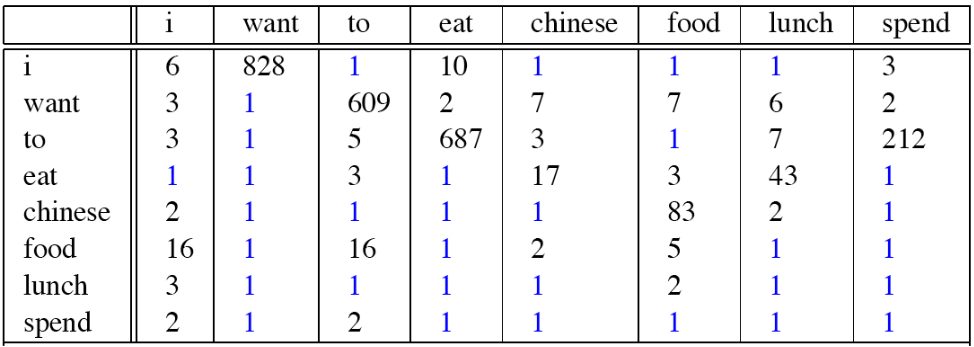
\includegraphics [scale=0.45] {laplace_smoothed_bigram_counts.png}
        \end{figure}
	
\end{frame}
%------------------------------------------------


\begin{frame}
    \onehalfspacing
        \frametitle{Berkeley Restaurant Corpus}
        {\Large Laplace-smoothed bigrams} \vspace{-2em}
        \begin{center} 
            \[ P^*(w_n | w_{n-1}) = \frac{c(w_{n-1} w_n) + 1}{c(w_{n-1}) + V} \]
          \end{center}
        
            \begin{figure}
                \centering
                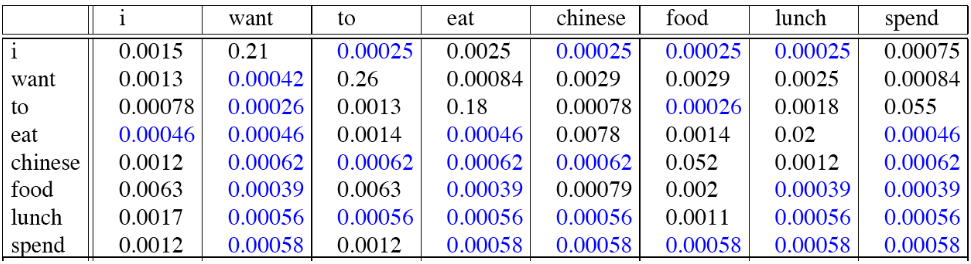
\includegraphics [scale=0.45] {laplace_smoothed_bigrams.png}
                
            \end{figure}
        
    \end{frame}
%------------------------------------------------

\begin{frame}
    \onehalfspacing
        \frametitle{Berkeley Restaurant Corpus}
        {\Large Reconstituted counts} \vspace{-2em}
        \begin{center} 
            \[ c^*(w_{n-1} w_{n}) = \frac{[ C(w_{n-1} w_n) + 1] \times C(w_{n-1})} {C(w_{n-1}) + V} \]
          \end{center}
        
            \begin{figure}
                \centering
                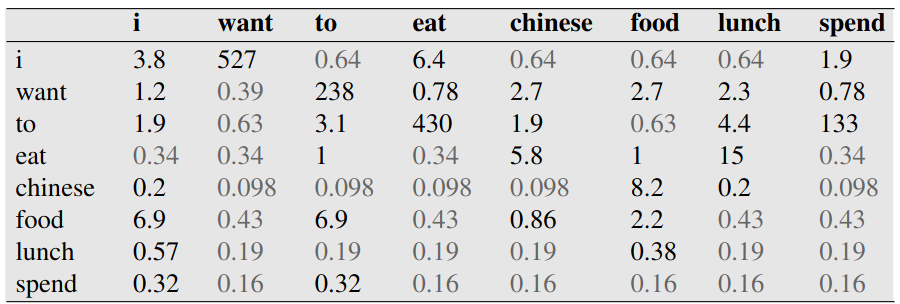
\includegraphics [scale=0.5] {add_one_reconsituted_counts.png}
                \caption{Add-one reconstituted counts for eight words (of V = 1446) in the BeRP corpus
                of 9332 sentences. Previously-zero counts are in gray}
            \end{figure}
    \end{frame}
%------------------------------------------------
\begin{frame}
\onehalfspacing
	\frametitle{Berkeley Restaurant Corpus}
    \begin{minipage}{0.5\textwidth}
        \begin{block}{}
            Compare with raw bigram counts
        \end{block}
    \end{minipage}

	\begin{figure}[h]
        \centering
        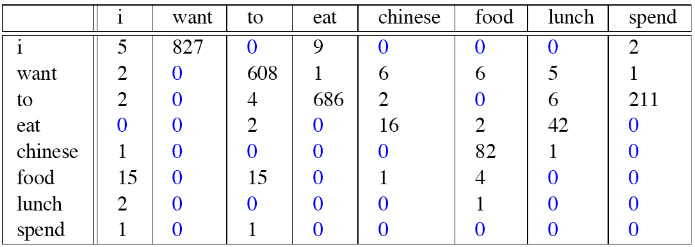
\includegraphics [scale=0.45] {raw_bigram_counts.png}
        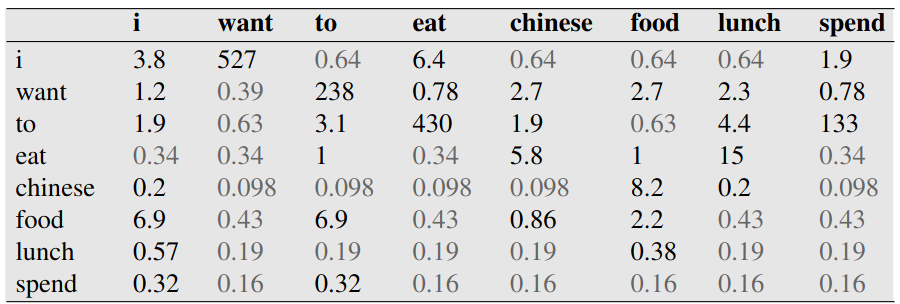
\includegraphics [scale=0.45] {add_one_reconsituted_counts.png}
    \end{figure}
\end{frame}

%------------------------------------------------
\subsection{Add-k smoothing}
\begin{frame}
    \onehalfspacing
        \frametitle{Add-k smoothing}
        {\Large Instead of adding 1 to each count, we add a \textbf{fractional} count $k$ (.5? .05? .01?). } \vspace{-2em}

        \begin{center} 
            \[ P^*_{Add-k} (w_n | w_{n-1}) = \frac{C(w_{n-1} w_n) + k}{C(w_{n-1} + kV)} \]
          \end{center}

       \begin{block}{}
        Add-k smoothing requires that we have a method for choosing $k$; this can be done, for example, by optimizing on a \textbf{devset}.

       \end{block}
    \end{frame}
    
%------------------------------------------------


\begin{frame}
\onehalfspacing
	\frametitle{Add-1 estimation is a blunt instrument}
    {\Large So add-1 isn’t used for N-grams:}
    \begin{itemize}
        \item {\large We’ll see better methods}

    \end{itemize}
    \vspace{3em}
    {\Large But add-1 is used to smooth other NLP models}
    \begin{itemize}
        \item {\large For text classification}
        \item {\large In domains where the number of zeros isn’t so huge.}
    \end{itemize}

   
\end{frame}

%------------------------------------------------
\subsection{Backoff and Interpolation}
\begin{frame}
    \onehalfspacing
        \frametitle{Backoff and Interpolation}
        {\Large Sometimes it helps to use \textbf{less} context}
        \begin{itemize}
            \item {Condition on less context for contexts you haven’t learned much about}
    
        \end{itemize}
        
        \begin{minipage}{0.5\textwidth}
            \begin{block}{\center{Backoff}}
                \begin{itemize}
                    \item Use trigram if you have good evidence
                    \item Otherwise bigram or unigram
                \end{itemize}
            \end{block}
        \end{minipage} \hspace{10}
        \begin{minipage}{0.45\textwidth}
            \begin{block}{\center{Interpolation}}
                \begin{itemize}
                    \item Mix unigram, bigram, trigram \\ \vspace{5}
                    \hphantom{fndfjndnjfjnd}
                \end{itemize}
            \end{block}
        \end{minipage}
    
        \bigskip

        % \begin{minipage}{0.4\textwidth}
        %     \begin{block}{}
        %         Interpolation works better
        %     \end{block}
        % \end{minipage}
       
    \end{frame}

%------------------------------------------------

\begin{frame}
    \onehalfspacing
        \frametitle{Liner Interpolation}
        {\Large Simple interpolation}
        \begin{minipage}{0.65\textwidth}
        \begin{center} 
            \[ \hat{P}(w_n | w_{n-2} w_{n-1}) = \lambda_1 P(w_n | w_{n-2} w_{n-1}) \\ \vspace{-1em}
                                                \hspace{7em} + \lambda_2 P(w_n | w_{n-1}) \\ 
                                                \hspace{4.5em} + \lambda_3 P(w_n) \]
          \end{center}
        \end{minipage}
        \hspace{10}
        \begin{minipage}{0.3\textwidth}
            \vspace{2em}
            \centering
            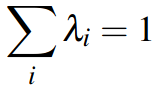
\includegraphics[scale=0.5]{sum_all_lambdas.png}
        \end{minipage}

        \vspace{3em}
        {\Large Lambdas conditional on context:}
        \begin{minipage}{0.75\textwidth}
        \begin{center} 
            \[ \hat{P}(w_n | w_{n-2} w_{n-1}) = \lambda_1 (w^{n-1}_{n-2}) P(w_n | w_{n-2} w_{n-1}) \\ \vspace{-0.5em}
                                                \hspace{7em} + \lambda_2 (w^{n-1}_{n-2}) P(w_n | w_{n-1}) \\ \vspace{0.5em}
                                                \hspace{4.5em} + \lambda_3 (w^{n-1}_{n-2}) P(w_n) \]
          \end{center}
        \end{minipage}
    
       
\end{frame}
    

%------------------------------------------------

\begin{frame}
    \onehalfspacing
        \frametitle{How to set the lambdas?}
        {\Large Use a \textbf{held-out} corpus}
        \begin{minipage}{0.75\textwidth}
           \centering
           
\includegraphics[scale=0.5]{held_out_corpus.png}
        \end{minipage}

        \vspace{3em}
        \begin{block}{Choose $\lambda$s to maximize the probability of held-out data:}
        \begin{itemize}
            \item Fix the N-gram probabilities (on the training data)
            \item Then search for $\lambda$s that give largest probability to held-out set: \\ \vspace{1em}
            \hspace{1.5em} $ \log{P(w_1 ... w_n | M(\lambda_1 ... \lambda_k))} = \sum_{i} \log{P_{M(\lambda_1 ... \lambda_k)} (w_i | w_{i-1})} $
        \end{itemize}
        \end{block}
    
       
    \end{frame}
    
    %------------------------------------------------

\begin{frame}
    \onehalfspacing
        \frametitle{Backoff}
        \begin{block}{In a \textbf{backoff} n-gram model}
            \begin{itemize}
                \item If the n-gram we need has zero counts, we approximate it by backing off to the (n-1)-gram.
                \item We have to discount the higher-order n-grams to save some probability mass for the lower order n-grams.
                \item If we don’t, the total probability assigned to all possible strings by the language model would be greater than 1.
            \end{itemize}
        \end{block}
    
        
\end{frame}

%------------------------------------------------


\begin{frame}
    \onehalfspacing
        \frametitle{Katz Backoff}
        {\Large We’ll need a function alpha to distribute this probability mass to the lower order n-grams.
        }

        \begin{equation*}
            P_{BO} (w_n | w_{n-N+1:n-1})=
            \begin{cases}
              P^*(w_n | w_{n-N+1:n-1}), & \hspace{-5em} \text{if}\ C(w_{n-N+1:n}) > 0 \\
              \alpha(w_{n-N+1:n-1}) P_{BO} (w_n | w_{n-N+2:n-1}), & \text{otherwise}
            \end{cases}
          \end{equation}
    
        
\end{frame}

%------------------------------------------------


\onehalfspacing
\begin{frame} % Use [allowframebreaks] to allow automatic splitting across slides if the content is too long
	\frametitle{Reference}
	
	\begin{thebibliography}{99} % Beamer does not support BibTeX so references must be inserted manually as below, you may need to use multiple columns and/or reduce the font size further if you have many references
		\footnotesize % Reduce the font size in the bibliography
		
		\bibitem[Stanford]{p1}
			Speech and Language Processing (3rd ed. draft)
			\newblock Dan Jurafsky and James H. Martin
			\newblock Part I: Fundamental Algorithms, \emph{Chapter 3: N-gram Language Models	}
			
		
	\end{thebibliography}
\end{frame}



%	CLOSING SLIDE
%----------------------------------------------------------------------------------------

\begin{frame} % The optional argument 'plain' hides the headline and footline
	\begin{center}
		{\Huge Thanks for listening!}
		
		\bigskip\bigskip % Vertical whitespace
		
		{\LARGE Q\&A section}
	\end{center}
\end{frame}
%------------------------------------------------


\end{document}
